\chapter{Background}
\label{ch2}
\Forf{T} relies on the research from many fields of study in both mathematics and computer science. In this chapter we will briefly examine the underlying theory, concepts, and frameworks upon which we rely to convey the ideas presented in this thesis and bring to fruition the work invested in designing and developing \forf{t}.
\todoReword{Elaborate like a teasing summary}
%
%
%
%
%
\section{Basic Theory}\todoReword{theoretical foundation}
The following is an abbreviated list of the important theoretical concepts used in the chapters to follow. These include concepts from set theory, geometry, and topology.
%
\subsection{Set Theory}
A set is one of the most fundamental concepts in mathematics. Informally, a set is a collection of distinct objects, and is also itself considered to be an object. In this thesis, sets are denoted using capital, calligraphic letters, such as: $\bM$, $\bP$, $\bT$, and $\bF$. 
%
\subsubsection{Set Definitions}
A set may be defined using ``intensional definitions'' or ``extensional definitions''. An intensional definition uses semantic rules and symbols, where each symbol can be translated into words so that the definition may be coherently read aloud. For example:
\begin{equation}
	\bP := \left \{\:\bp_v \mid v \in \mathbb{N}, \;\text{and}\; 1\leq v \leq v_{max}\:\right \}
\end{equation}
which should be read as, ``$\bP$ is defined as the set of all points $\bp_v$, such that the index $v$ is a member of the set of natural numbers, and $v$ is a number from 1 to the maximum index of points in the set.''

The other option, extensional definition, is denoted by enclosing the list of members in curly brackets, and optionally invoking an ellipsis (``\dots'') for continuing into infinity. For example:
%
\begin{equation}
	\mathbb{N} = \left \{\:0,\,1,\,2,\,3,\,\ldots\:\right \}
\end{equation}
%
A set member is allowed to be listed two or more times in a definition, for example $\left \{\:4,\,2,\,2\:\right \}$. However, it is identical to the set $\left \{\:4,\,2\:\right \}$ per the axiom of extensionality\todoResearch{Zermelo–Fraenkel set theory., Axiom of extensionality, logical extensionality}, which states that two definitions of sets, which differ only in that one of the definitions lists members multiple times, define the same set.
%
\subsubsection{Special Sets}
There exists some sets which are used in mathematical literature with such frequency as to demand their own standardized symbols. In this thesis\todoReference{defineSetofNaturalNumbers}, we have already encountered $\mathbb{N}$, which denotes the set of all natural numbers.
%
\subsubsection{Cardinality}
Denoted as $|\bM\,|$, the cardinality of a set is the number of its members, so if $\bM = \left \{\,\bP,\,\bT\right \}$, then $|\bM\,| = 2$.
%
\subsubsection{Membership \& Relational Operators}
If an object is said to be a member of a set, it is written with the symbol $\in$ and expressed as either belonging to or being an element of the set. Similarly, a set may be the subset of another set, written with the symbol $\subseteq$, meaning that every member of the first set is also a member of second set. A superset works exactly in reverse, written with the symbol $\subseteq$, it is the identity where every member of the second set is also a member of first set. In mathematical notation, those examples are written as\footnote{The negative operators also exists as $\notin$ and $\nsubseteq$}
\begin{align}
	B & \in \left \{A,\,B,\,C\right \} \\
	\left \{A,\,B\right \} & \subseteq \left \{A,\,B,\,C\right \} \\
	\left \{A,\,B,\,C\right \} & \supseteq \left \{A,\,B\right \}
\end{align}
%
\subsubsection{Binary Operations}
Among all the basic binary operations one can perform on a set\footnote{which are the union, intersection, complement, and Cartesian product}, in this thesis, we exclusively use the union operation, denoted as $\cup$, whose output is the set of all objects that are members of either set, or both. For example:
\begin{equation}
	\left \{0,\,1,\,2\right \} \cup \left \{2,\,3,\,4\right \} = \left \{0,\,1,\,2,\,3,\,4\right \}
\end{equation}
\todoReword{would look better to have words here}
%
%
%
\subsection{Geometry}
As vast and encompassing is geometry as a field of study, of paramount importance for \forf{t} are interpolation, the concept of a geodesic disc, and the characteristics of a circle sector.
%
\subsubsection{Interpolation}
Simply stated, interpolation is a method of constructing new data points within the range of a discrete set of known data points, such as those points used in \tdd{}. There exist a large variety of methods for interpolating different kinds of data\todoCitation{different kinds of interpolation}, but as an introduction, let us first consider linear interpolation, which is simple to calculate\footnote{however can become imprecise in relation to the square of the distance between the data points.}\todoCitation{footnote:error of linear interpolation} and can be extended for n-dimensions\todoCitation{n-dimensional linear interpolation}.

Given the two data points in $\mathbb{R}^2$, $(x_a, y_a)$ and $(x_b, y_b)$, the so called interpolant of a point located at\todoReword{don't use point located at, maybe value sampled at instead?} $x_c$ can be calculated as
\begin{equation}
	y_c = y_a + (y_b - y_a) \frac{x_c - x_a}{x_b - x_a}
	\label{eq:interpolationGeneral}
\end{equation}
To illustrate the concept, consider the two points $(1, 4)$ and $(3, 1)$, then find the interpolant of a point located at $x = 2$\todoReword{don't use point located at, maybe value sampled at instead?}
\begin{align}
	y_c & = 4 + (1 - 4) \frac{2 - 1}{3 - 1} \\
	& = 4 + -3 \frac{1}{2} \enspace = \enspace  2.5	
	\label{eq:interpolationSpecific}
\end{align}
So the value halfway between the two given points is interpolated to be $(2, 2.5)$, which is halfway between as expected. Interpolation becomes even more intuitive when seen graphically as shown in Figure~\ref{fig:interpolation}.
\begin{figure}
\ffigbox
	{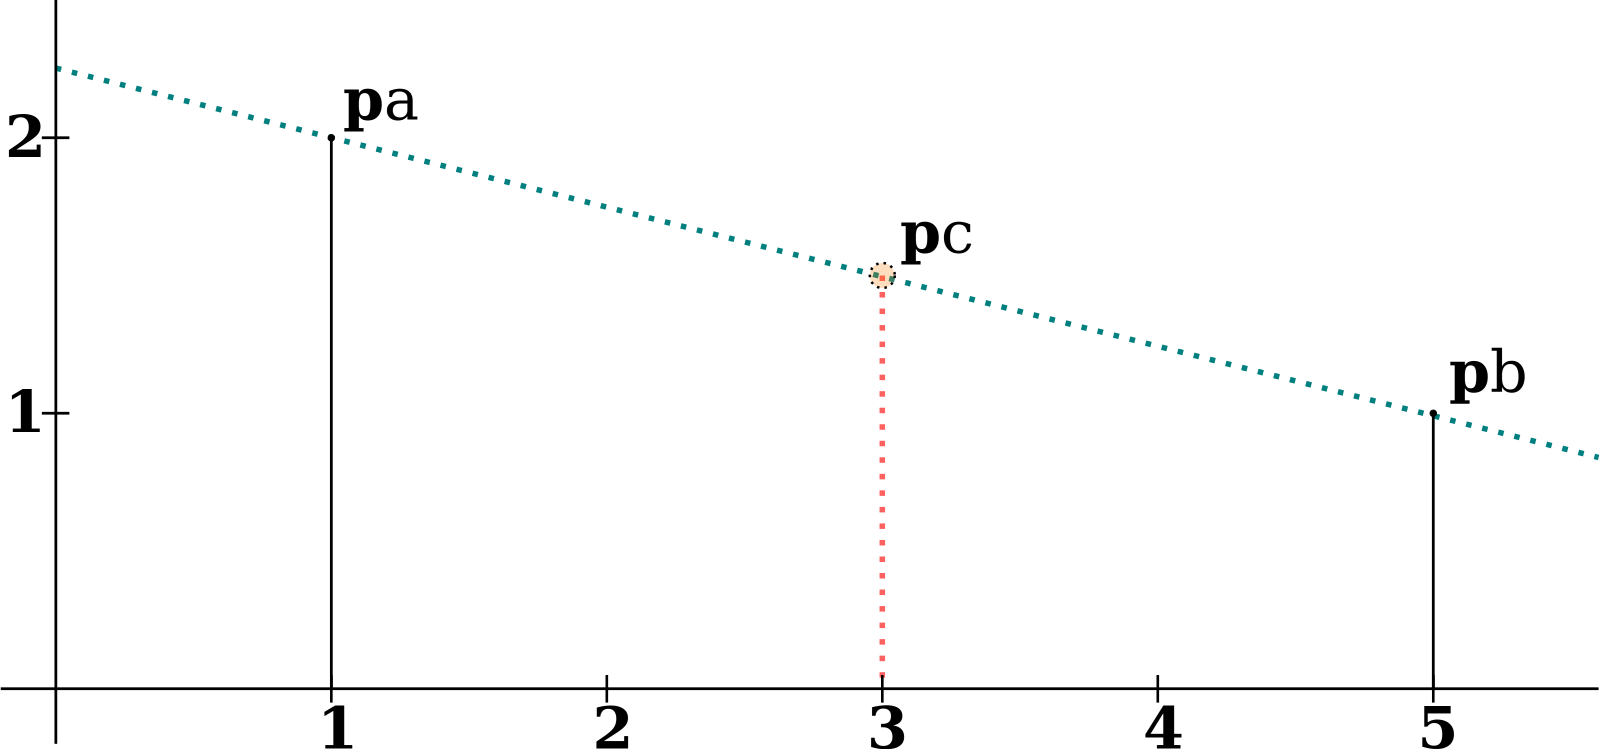
\includegraphics[width=1.0\linewidth]{figures/interpolation.png}}
	{\caption[Interpolation between two points in $\mathbb{R}^2$]{$\bp_c$ is interpolated as a value between $\bp_a$ and $\bp_b$}\label{fig:interpolation}}
\end{figure}
%
\subsubsection{Circle Sectors}
A circular sector, or circle sector, is the portion of a disc enclosed by two radii and an arc. In general, the larger area is known as the major sector, however \forf{t} is only concerned with the area of other, smaller area, known as the minor sector, but from here will be abbreviated as the circle sector, or even more simply, the sector.

In the Figure~\ref{fig:circleSector}, $\alpha$ is the central angle\footnote{expressed in radians, as all angles are in this thesis}, r the radius of the circle, and L is the arc length of the minor sector.
\todoResearch{https://en.wikipedia.org/wiki/Circular\_sector}
\begin{figure}
\ffigbox
	{\includegraphics[width=1.0\linewidth]{example-image-16x9.png}}
	{\caption[Regular Planar and Irregular Non-planar Neighborhoods in $\mathbb{R}^2$]{A circle sector}\label{fig:circleSector}}
\end{figure}

As the sector is defined entirely the central angle and the circle's radius, the area of the sector can be given as
\begin{equation}
	A = \pi r^2\frac{\alpha}{2\pi} = \frac{r^2\alpha}{2}
	\label{eq:areaOfCircleSector}
\end{equation}
because the area can be obtained by multiplying the circle's total area by the ratio of the sector's central angle $\alpha$, and $2\pi$, the total angle of the circle in radians.
%
%
%
\subsection{Topology}
Topology is the mathematical study of the properties of space that are preserved through deformations, twistings, and stretchings of objects\footnote{but not tearing or gluing}, which developed as a field of study from geometry and set theory through analysis of concepts such as space, dimension, and transformation. For example, a circle is topologically equivalent to an ellipse, because it can be deformed by stretching.~\cite{Weisstein19c} Of the major concepts, this thesis is most concerned with manifolds and neighborhoods.
%
\subsubsection{Manifolds}
A manifold is a topological space that is locally, but possibly not globally, Euclidean; a concept that is central to many parts of geometry because it allows complicated structures, such as the triangle mesh, to be described and understood in terms of the simpler, local topological properties. In general, that means that a manifold is an $n$D-subset of an Euclidean space $\mathbb{R}^{>n}$.~\cite[p.~199]{Mara12} For example, 1-dimensional manifolds in $\mathbb{R}^{2}$ include lines and circles, and 2-dimensional manifolds in $\mathbb{R}^{3}$, also called surfaces, can include commonly-known shapes such as the plane, the sphere, and the torus, but also of prime importance for this thesis, the triangle mesh.
%
\subsubsection{Neighborhoods}
A neighborhood is also one of the basic concepts of topology. Intuitively speaking, a neighborhood of a point is a set of points containing that point where one can move in any direction without leaving the set. While determining the neighborhood is trivial for 1-dimensional manifolds, and relatively simple to regular surfaces, such as a 2D-images whose pixels have at most four neighbors in orthogonal direction with a geometric distance of 1, as well as four neighbors at the diagonal directions with a geometric distance of $\sqrt{2}$, determining the neighborhood becomes more complicated for non-planar, irregular surfaces like those found in \tdd{}. With those surfaces, one must determine the set of neighbors using the definition of the connected triangular faces. The details of which are covered in detail in Section:~\ref{ch2s3ssNRN}, after the necessary topics regarding \tdd{} have already been discussed.

Figure~\ref{fig:neighborhoods} illustrates the difference between the neighborhood of a point in a two kinds of regular meshes, and the neighborhood of a point in an irregular, non-planar mesh as found in \tdd{}.
%
\begin{figure}
\ffigbox
	{\includegraphics[width=1.0\linewidth]{example-image-16x9.png}}
	{\caption[Regular Planar and Irregular Non-planar Neighborhoods in $\mathbb{R}^2$]{Neighborhoods in differing manifolds in $\mathbb{R}^2$ (a) a regular, planar mesh (b) a regular, planar triangle mesh (c) an irregular, non-planar triangle mesh, typical of acquired \tdd{}}\label{fig:neighborhoods}}
\end{figure}
%
Notice the completely arbitrary shape and size of the 1 ring neighborhood found in the (c) acquired mesh. From this observation is where the motivation behind \forf{t} came.
%
%
%
%
%
\section{\tdd}
\label{ch2s3}
\todoStyle{the 3 in \tdd{} looks too small}
The data upon which one convolves \forf{t} is called \tdd\todoCitation{\tdd{} name origin, BB82 from Mara12}. As described in Section~\ref{ch2s3ssM}, \tdd{} consists primarily of a single mesh $\bM$, which is the superset of $\bP$, a set of points, and the set $\bT$ consisting of triangular faces, each to be covered in Sections~\ref{ch2s3ssP} and~\ref{ch2s3ssF} respectively. \tdd{} also comes in two distinct flavors depending on its origin: acquired or synthetic, as discussed in Section~\ref{ch2s3ssAVS3}. The data can also include a texture map and other various types of information stored as scalar or vector fields, as elaborated on in~\ref{ch2s3ssFV}.
%
\subsection{Points}
\label{ch2s3ssP}
A point $\bp$ is the most primitive element of \tdd{}. "Point" is the abbreviated form of "measuring point", and is also known in other fields of study as a vertex, or a position vector $\in \mathbb{R}^3$\todoCitation{other names for a point}. A point is defined by the 3-dimensional Cartesian coordinates $x$, $y$ and $z$, and in \tdd{}, points are generally unique and not required to be in any particular order. In this thesis, a point is addressed using several different subscripts, depending on the context.

Index $v$ is the globally unique index, with which we can define the set
\begin{equation}
	\bP := \left \{\:\bp_v \mid v \in \mathbb{N}, \;\text{and}\; 1\leq v \leq v_{max}\:\right \}
	\label{eq:defineSetOfPoints}
\end{equation}
where $v_{max}$ is the maximum index of points in the data, and is equivalent to the cardinality of the set of points $|\bP|$.%
\nomenclature[ab]{$\bP$}{the set of points $\bp$ in $\bM$}%
\nomenclature[ac]{$\bp_v$}{a specific point in $\bP$}%

Please note that the indices in Equation~\ref{eq:defineSetOfPoints} begin with 1. This is significant because of the discordant conventions between addressing the first element of a data structure with 0 in programming languages such as C++ and python, versus addressing first elements with 1, as is the standard for mathematical literature. Because this thesis should indeed be considered mathematical literature, we will always start indices at 1, and only use index 0 for special cases. For example, $\bp_0$ is used to represent the defining center point of a one-ring neighborhood\todoReference{neighborhoods section}.
\todoStyle{This could be a long footnote.}

Otherwise,
% when referencing to a point by its index within a specific one-ring neighborhood, we will use $\bp_k$, and %
 when referencing to a point within a particular face or neighborhood, the three corners can be referenced indirectly as $\bp_i$\footnote{or generally as $\bp_a$, $\bp_b$, $\bp_c$ in the case of Equation~\ref{eq:defineEdgeLengthFace}, or in the case of a nested loops: as $\bp_k$ in Algorithm~\ref{alg:serialBuildNeighborhoods}, and $\bp_j$ in Algorithm~\ref{alg:serialCompute}}, $\bp_{\sipo}$, and $\bp_{\sipt}$, or directly as $\bp_0$, $\bp_1$, and $\bp_2$.~\cite[p.~25]{Mara12}%
\todoReword{ensure footnote indice remain correct}%
\nomenclature[ad]{$\bp_i$}{also $\bp_{\sipo}$, and $\bp_{\sipt}$; one of three indirectly referenced points comprising a face}%
%
\subsection{Faces}
\label{ch2s3ssF}
Faces are the another primitive element of \tdd{}. As we are working exclusively with triangular meshes~\cite[p.~26]{Mara12}, we define a face $\bt$ by the totally ordered~\cite{Weisstein19a} set of three distinct points, which we will index in clockwise order~\cite[p.~4]{Mara17}.

It is worth mentioning here that many software packages, such as the GigaMesh Framework~\cite[p.~89]{Mara12}, may expect counter-clockwise ordering of indexes. \todoResearch{does the "right-hand-rule apply here?"} This is significant because the ordering provides an orientation by which visualization software can apply texture and/or lighting. The only mathematical significance of the ordering is the sign of the area of a face, and totally inconsequential when the absolute value is expected, as shown by\cite[p.~2]{Braden86}. This is yet another example of the difference between the conventions of mathematical literature versus those of computer science. And again, because this thesis should indeed be considered mathematical literature, we will continue to follow the conventions of mathematical literature.
\todoStyle{probably better as a footnote}

The triangular faces are addressed using the global index $k$, and each has three implicit edges whose descriptions are elaborated upon in Section~\ref{chBsEL}.
\begin{equation}
	\bt_k := \left \{\bp_0, \bp_1, \bp_2\right \} \equiv \left \{A_k, B_k, C_k\right \} \hspace{20pt}\text{abbreviated:}\hspace{20pt} \bt = \left \{A, B, C\right \}
	\label{eq:defineSetOfFaces}
\end{equation}%
\nomenclature[ae]{$\bt_k$}{a specific face in $\bT$}%
%
\begin{figure}[]
\ffigbox
	{\includegraphics[width=0.8\linewidth]{example-image-16x9.png}}
	{\caption[A Triangular Face]{A triangular face showing points, edges, and orientation}\label{fig:facesOfAMesh}}
\end{figure}
%
The set of triangular faces is defined as
\begin{equation}
	\bT := \left \{\:\bt_k \mid k \in \mathbb{N}, \;\text{and}\; 1\leq k \leq k_{max}\:\right \}
	\label{eq:defineSetOfFaces}
\end{equation}
where $k_{max}$ is the maximum index of faces in the data, and is equivalent to the cardinality of the set of faces $|\bT|$.%
\nomenclature[ad]{$\bT$}{the set of faces $\bt$ in $\bM$}%

%
\subsection{Edge Lengths}
\label{chBsEL}
As illustrated in Figure~\ref{fig:facesOfAMesh}, each triangular face is implicitly composed of three edges. Despite the fact that an edge is not typically\footnote{Other data structures, such as the Winged-Edge~\cite[p.~1]{Baumgart75}, may use edges as a primitive element} a primitive element of \tdd{}, we will endeavor to define the length of an edge $\ell$, because edge lengths are of particular significance for both the design and implementation of \forf{t}.

When in the context of a particular face $\bt_k$, we will use the single index $i$ to define the length
\begin{equation}
	\ell_a := |\bp_b - \bp_c| \enspace:\enspace \left \{\:\bp_a, \bp_b, \bp_c\:\right \} = \bt_k
	\label{eq:defineEdgeLengthFace}
\end{equation}%
\nomenclature[af]{$\ell_i$}{the length of edge $\ell_i$ of a specific face}%
 
and the double indices $v,k$, when an edge length is referenced in relation to specific point $\bp_v$ and its neighbor $\bp_k$
\begin{equation}
	\ell_{v,k} := |\bp_k - \bp_v|
	\label{eq:defineEdgeLengthPoint}
\end{equation}%
\nomenclature[ag]{$\ell_{v,k}$}{the length of distance from point $\bp_v$ to $\bp_k$}%
Please note the similar notation for the cardinality of a set $|\bP|$, to that for the calculation for the length of the edge $|\bp_k - \bp_v|$ as defined in Equation~\ref{eq:defineEdgeLengthPoint}. While cardinality is simply the count of elements in the set, the length is calculated as the L2-norm of the referenced vector.~\cite[p.~26]{Mara12}
%\begin{align}
\begin{equation}
\begin{aligned}
	|\bp_k - \bp_v| & = \lVert\bp_k - \bp_v\rVert_2 \\
					& = \sqrt{(x_k-x_v)^2 + (y_k-y_v)^2 + (y_k-y_v)^2}
	\label{eq:defineEdgeLengthCalc}
\end{aligned}
\end{equation}
%\end{align}
\todoResearch{can I avoid sqrt altogether by performing entire algorithm squared?}
%
\subsection{Meshes}
\label{ch2s3ssM}
In \tdd{}, a mesh $\bM$ is the digital representation of a discrete manifold embedded in $\mathbb{R}^3$, and is typically\footnote{except in the case of specifically designed synthetic data~\ref{Experiments}} 2D-non-planar\todoStyle{in 2D, the 2 looks small} and comprised of non-regular, triangular faces composed of connected points.~\cite[p.~25]{Mara12} A mesh is the superset defined as
\begin{equation}
	\bM := \left \{\bP,\:\bT\right \}
	\label{eq:defineMesh}
\end{equation}%
\nomenclature[aa]{$\bM$}{a mesh; the superset including the sets of all points $\bp$ and faces $\bt$}%
with the set $\bP$ consisting of points, and the set $\bT$ consisting of triangular faces.

Many 3D-scanners produce point clouds\todoCitation{}{}, which as the name suggests, are comprised soley of a set of points $\bP$ and do not provide the set $\bT$. However, it is possible, and necessary for the production of a mesh, to perform a point set triangulation\todoCitation{}{} in order to connect $\bP$ into a set of triangle faces, enabling one to combine the two sets into a mesh~\cite[p.~26]{Mara12}. For example, during our experiments, we perform the well-known Delaunay triangulation\todoCitation{} in order to produce a mesh from a randomly generated point cloud\todoReword{add ref to experiments}.
%
\subsection{1-Ring Neighborhoods}
\label{ch2s3ssNRN}
It was mentioned in Section~\ref{ch2sBssT}, that determining the neighborhood of a point $\bp_v$ is non-trivial. Having now examined the definitions of points, faces, and meshes, we can now formalize the 1-ring neighborhood in \tdd{} as
\begin{equation}
	\bN_v := \left \{\;\widetilde{\bp_v}\;|\;\left \{\,\widetilde{\bp_v},\,\bp_v\right \} \subseteq \bt \quad \forall \bt \in \bT\;\right \}
	\label{eq:defineNeighborhood}
\end{equation}%
\nomenclature[ai]{$\bN_v$}{the set of points comprising the 1-ring neighborhood about $\bP_v$}%
\nomenclature[aj]{$\widetilde{\bp_v}$}{a 1-ring neighbor of $\bP_v$}%
\todoStyle{use a big $\mathring{\bp_v}$ instead of $\widetilde{\bp_v}$}
which said another way, means that the neighborhood $\bN_v$ is defined as the set of points $\widetilde{\bp_v}$ such that both $\widetilde{\bp_v}$ and $\bp_v$ are two points of a triangular face $\bt$, for all faces in the mesh.

The set of points $\widetilde{\bp_v}$, as illustrated in Figure~\ref{fig:neighborhoods}, which comprise $\bN_v$, belong to what is known as a 1-ring neighborhood of $\bp_v$, because are directly connected with the center point $\bp_v$ and so are considered to have a relative distance of 1 within the graph\todoReword{do I need graph theory in basic theory section?} of the mesh. The 1-ring can be extended to a 2-ring by taking the union of the neighborhood $\bN_v$ with each neighborhood of each 1-ring neighbor $\widetilde{\bp_v}$, which adds points having the relative distance of 2 within the graph. This iterative concept can be repeated k times and the neighborhood is than referred to as k-ring. Unfortunately, the relative distance within the graph can not be assumed equal to the geometric distance nor geodesic distance, regardless of that fact, it is used throughout the literature – especially in the field of Computer Graphics.~\cite[p.~29]{Mara12}

Our solution for computing \forf{t} in light of these complications is explained in greater detail in Chapter~\ref{}, later in this thesis.
%
\subsection{Acquired vs Synthetic \tdd{}}
\label{ch2s3ssAVS3}
The corpus of \tdd{} exists in two flavors, acquired and synthetic data, with each being handily classifiable by the fashion in which it was generated, and the characteristics innate to those techniques.

Acquired \tdd{} is typically captured as a point cloud utilizing various methods, such as: LiDAR (Light Detection and Ranging), Structured Light, or Structure from Motion~\cite[p.~19]{Mara12}. Then the data is exported from software packages accompanying the 3D-scanners as either just the point cloud as a simple set of points $\bP$, or optionally as a triangle mesh $\bM$, described by one or more scalar-fields. Acquired \tdd{} also often consists upwards of a million points and as many as twice that number of faces\todoReference{the interesting experimental finding about face to vertex ratio; add as a footnote}. These exported meshes ~\cite[p.~25]{Mara12} uniformly contain noise and may exhibit other complexities for analysis, such as: non-manifold points, multiple borders and holes in the surface, inverted face orientation, non-manifold edges, and agglutination or degenerate faces. ~\cite[p.~28-32]{Mara12}

Conversely, synthetic \tdd{} is artfully crafted to obey the constraints of being a good mesh\todoReword{define a good mesh here}, without the complexities exhibited by acquired data. When modeling 3-dimensional objects, synthetic \tdd{} can require significantly less memory for storage, as simplifications can be made for large regular surfaces. For example, even the largest flat, rectangular surface can be modeled with only four points and two faces, whereas the acquired data methods require that the Nyquist–Shannon sampling theorem\todoCitation{Nyquist Shannon Theorem} be obeyed for the smallest detectable feature throughout the entire surface.~\cite[p.~19]{Mara12}~\cite[p.~3]{Mara17}

For our experiments, we created another kind of synthetic \tdd{} which does not model a 3D-object. Instead, these synthetic-mesh generators produce different types of tessellations on arbitrarily large, planar surfaces, accompanied by a configurable scalar-field of function values.\todoReword{reference experiments}
%
\subsection{Function Values}
\label{ch2s3ssFV}
In addition to the 3 Cartesian coordinates, a point may often contain other relevant data in the form of scalar fields, or when taken together, vector fields. This information, which is stored at each point $\bp$, often includes data regarding: RGB color, material type, reflectivity, transparency, quality, confidence, or the resulting function values from an analytical filter such as the Multi-Scale Integral Invariants (MSII) filter~\cite[p.~21]{Mara12}, but can be extended to include data important to other fields of study, such as: infrared or ultraviolet light, temperature, rainfall, population, crime-rates, etc; essentially, any kind of data that may be measured at a point. 

\forf{T} is agnostic to the meaning of information represented by the data, therefore, it can similarly process any such function values stored as a scalar field. However, because the filter was designed to only convolve scalar fields, any multi-dimensional data, such as RGB color, must be processed individually as independent scalar fields.\todoReference{future work/applications} The result is that we can define a scalar field simply as a set of function values.
%
\begin{equation}
	\bF := \left \{\: f_v \mid v \in \mathbb{N}, \;\text{and}\; 1\leq v \leq v_{max} \:\right \}
	\label{eq:defineSetOfFunctionValues}
\end{equation}%
\nomenclature[ak]{$\bF$}{the set of function values $f$; a scalar field}%
\nomenclature[al]{$f_v$}{a specific function value in $\bF$, corresponding to $\bp_v$}%
%
This definition shares the indices $v$ and $v_{max}$ with the definition for a set of points, Equation~\ref{eq:defineSetOfPoints}. Indeed, it is a fact that the cardinality of $|\bF|$ must be equal to $|\bP|$
\begin{equation}
	|\bF| \mbeq |\bP|
\end{equation}
because function values are only stored alongside the Cartesian coordinates, 1-for-1 with points, due to \tdd{} existing as a discrete manifold.\todoResearch{storing data between points on a discrete manifold}
%
%
%
%
%
\section{Architectures of Concurrency}
%
\subsection{Serial Computation \& Threads}
%thread can be identified using a one-dimensional, two-dimensional, or three-dimensional thread index, forming a one-dimensional, two-dimensional, or three- dimensional block of thread, called a thread block. This provides a natural way to invoke computation across the elements in a domain such as a vector, matrix, or volume. However, a kernel can be executed by multiple equally-shaped thread blocks, so that the total number of thread is equal to the number of thread per block times the number of blocks. thread blocks are required to execute independently: It must be possible to execute them in any order, in parallel or in series. This independence requirement allows thread blocks to be scheduled in any order across any number of cores as illustrated by Figure 5, enabling programmers to write code that scales with the number of cores. [7, p. 2.2]
\todoReword{found elsewhere in thesis}
%
\subsection{Multi-threaded Computation}
%Processors through Supercomputers and Data Centers
%
\subsection{Concurrency vs Parallelism}
%
\subsection{Flynn's taxonomy}
1.1	Single instruction stream single data stream (SISD)
1.2	Single instruction stream, multiple data streams (SIMD)
1.3	Multiple instruction streams, single data stream (MISD)
1.4	Multiple instruction streams, multiple data streams (MIMD)
%
\section{CUDA: An interface for GPGPU implementation}
\subsection{CUDA C Runtime}%3.2. CUDA C Runtime}
\subsubsection{Explicit Synchronization}%3.2.5.5.3. Explicit Synchronization}
\subsection{Versioning and Compatibility}%3.3. Versioning and Compatibility}
\subsection{Hardware Implementation}%4. Hardware Implementation}
\subsubsection{SIMT Architecture}%4.1. SIMT Architecture}
\subsection{Host Memory and Device Memory}
\subsection{Versions <9, vs >= 9}
%
%
%
%
%
\section{Evaluation and Analysis of Concurrent Algorithms}~\cite[p.~330]{Lang17}
%Multi-node out of scope?!
%
\subsection{Timing}
%\begin{equation}
%	N = input size (num. ops)
%	P = processor count
%	Ts(N) = Sequential execution time
%	Tbest(N) = Optimal execution time
%	TP(N, P) = Parallel runtime
%\end{equation}
%
\subsection{Speedup, efficiency}
%	Speedup:
%S(N, P) = Tbest(N)/TP(N, P)

%	Efficiency:
%E(N, P) = Tbest (N)/PTP(N, P) = S/P

%	Costs:
%C(N, P) = PTP(N, P)
%
\subsection{Degree of Parallelism}
%	0 < q < 1 is the sequential part
%	1-q = is the parallelizable part
%
\subsection{Iso-efficiency}
%	WK(P) = iso-efficient if it fulfills:
%	TO(WK(P), P) = KWK(P)~\cite[p.~350]{Lang17}
%
\subsection{Scalability}
%	A parallel system is called scalable only if in has an iso-efficency function
%
%
%
%
%
\section{Summary}
%
